% Compile from docs/paper with pdflatex (IEEEtran required).
% All numbers come from benchmarks/results/oscd_results_v2.json.
% Citation slots are deliberate placeholders; see TODO_CITATIONS.md.
\documentclass[conference]{IEEEtran}
\usepackage{graphicx}
\usepackage{booktabs}
\usepackage{longtable}
\usepackage{amsmath}
\usepackage{url}
\usepackage[hidelinks]{hyperref}

\title{Transparent Sentinel-2 Change Detection as Decision Support:\\
A Reproducible OSCD Benchmark of Spectral Rules and a Learned Baseline}

\author{\IEEEauthorblockN{Author and affiliation to be completed}
\IEEEauthorblockA{Anonymous review version --- do not submit as-is}}

\begin{document}
\maketitle

\begin{abstract}
Operational change detection is often presented as a model-selection problem,
while deployed tools also need inspectable rules, bounded claims and reproducible
failure modes. We report a small, fully specified benchmark of a Sentinel-2
decision-support tool on the official OSCD urban-change test split. The system
combines NDVI/NDBI difference rules, cloud/shadow masking, a minimum mapping
unit and optional radiometric normalisation; a CNN baseline trained on aerial
imagery is evaluated under the same protocol. Thresholds and CNN preprocessing
were selected on the 14 training cities only. On the ten test cities, a
percentile spectral rule reached pooled F1 0.1176 (precision 0.2419, recall
0.0777) against a true change fraction of 5.17\%, while a hardcoded rule reached
F1 0.0782. Otsu thresholding predicted 67.35\% of pixels as changed and is
therefore reported by overall accuracy (0.3439), not by F1 alone. The CNN
produced near-empty predictions (pooled F1 0.0007 for the train-selected
variant), which we report as negative transfer rather than tune away. Per-city
F1 ranges from 0.0005 to 0.2481 for the percentile rule, so the aggregate hides
substantial variation. We describe a preregistered, validation-only protocol
for future improvements and explicitly leave its test score uncomputed. The
paper contributes an auditable negative result and an implementation pattern
for systems that must state what they do not validate.
\end{abstract}

\begin{IEEEkeywords}
Sentinel-2, change detection, OSCD, spectral indices, reproducibility,
decision support, negative transfer.
\end{IEEEkeywords}

\section{Introduction}
Satellite change detection is used to prioritise site visits, screen land-cover
transitions and communicate observations. In those settings a single accuracy
number is not enough: an operator needs to know which pixels were excluded, how
thresholds were chosen, which scenes were used, what the tool does not detect,
and whether a result was ever tested on independent labels. Deep models can
improve benchmark scores, but they can also fail silently when the deployment
sensor or resolution differs from training.

This paper documents a deployed, browser-based Sentinel-2 analysis tool and a
reproducible evaluation of its spectral rules against the official OSCD test
split. The evaluation is deliberately conservative. Thresholds are selected on
training cities; cloud and shadow masks are reported; labels are urban change
only; and the learned baseline's poor transfer is reported as measured. We do
not claim a new method or a top benchmark score. The contributions are an
end-to-end auditable implementation, a train-only benchmark with disclosed
scoring history, and a preregistered validation protocol for changes that have
not been scored on the test split.

The remainder of the paper reviews related work (Section~II), describes the
data and task (Section~III), the methods (Section~IV), the protocol including
its two prior test-scoring events (Section~V), results (Section~VI), the
validation-only ablation that was not run in this checkout (Section~VII), and
the limits of the claims (Sections~VIII--X).

\section{Related Work}
\label{sec:related}
Work on satellite change detection spans benchmark datasets and supervised
models [CITE: OSCD dataset and baseline models], spectral-index and
threshold-based detection [CITE: spectral indices for change detection],
[CITE: Otsu thresholding], and deep architectures for bitemporal imagery
[CITE: deep learning change detection surveys]. OSCD specifically provides
Sentinel-2 urban-change pairs and a fixed train/test city split
[CITE: OSCD dataset and protocol]; reported scores in that literature are not
directly comparable to the simple rules evaluated here.

A second line concerns transfer and evaluation. CNNs trained on one sensor,
resolution or label ontology can lose accuracy on another
[CITE: cross-sensor and domain-shift change detection], and repeated use of a
fixed test split can inflate apparent progress
[CITE: test-set reuse and benchmark overfitting]. Preregistration, spatial
cross-validation and provenance are established practices in remote sensing
and beyond [CITE: preregistration], [CITE: spatial cross-validation],
[CITE: reproducibility and provenance in remote sensing]. The implementation
also draws on interactive Earth-observation tools and decision-support
interfaces [CITE: open change-detection tools and decision support].

The emphasis of this paper is not a new detector. It is a conservative,
auditable evaluation of simple rules and one mismatched CNN, plus an
implementation that exposes validation status and provenance alongside each
result. The combination may not be unique; \texttt{NOVELTY\_CHECKLIST.md}
records a shallow scan and prohibits a priority claim. The contribution is the
evidence and the reporting discipline, both of which are limited by the threats
in Section~\ref{sec:limitations}.

\section{Data and Task}
\label{sec:data}
\subsection{OSCD}
We use the official OSCD urban-change benchmark layout with 14 training cities
and 10 test cities [CITE: OSCD dataset and protocol]. Each city provides a
before/after Sentinel-2 pair and a binary change label. Labels cover urban
change; they do not provide a general land-cover or forest-loss reference. In
the v2 test rows, the pooled true change fraction is 5.17\% across 3,077,936
pixels, so overall accuracy is dominated by the unchanged class.

The benchmark layout used here does not include Sentinel-2 Scene
Classification (SCL) layers. Cloud and shadow exclusion is therefore applied by
the live tool but is not evaluated by the v2 benchmark. Any statement about
cloud-mask quality would be unsupported by these numbers.

\subsection{Images and preprocessing}
The spectral path decodes an RGB preview and an encoded NDVI/NDBI/SCL image
from the live service. The offline benchmark computes NDVI and NDBI from
reflectance bands (B04/B08 and B11/B08) and applies the same threshold logic.
%% The benchmark pipeline does not use SCL; the live path does.
For the CNN path, before/after RGB arrays are normalised with ImageNet
statistics and tiled for inference. Two preprocessing variants were evaluated:
\emph{joint percentile} (selected on training cities) and \emph{reflectance}
(the other variant). The provided checkpoint is described as trained on
0.5\,m aerial LEVIR-CD pairs [CITE: LEVIR-CD dataset], not on OSCD Sentinel-2
imagery; the checkpoint is not included in this checkout.

\section{Methods}
\label{sec:methods}
\subsection{Spectral indices and rules}
For a Sentinel-2 pixel with red ($R$), near-infrared ($N$) and short-wave
infrared ($S$) reflectance,
\begin{align}
\mathrm{NDVI} &= \frac{N-R}{N+R}, \\
\mathrm{NDBI} &= \frac{S-N}{S+N}.
\end{align}
The general rule flags a pixel when NDVI decreases by more than a threshold or
NDBI increases by more than a threshold. The hardcoded configuration used
$\Delta\mathrm{NDVI} < -0.30$ or $\Delta\mathrm{NDBI} > +0.30$, selected from a
training-city grid; both selected values sit at the edge of the search grid.
The percentile configuration thresholds the positive-change evidence at a
training-selected percentile (99.0). Otsu's method selects a threshold from the
change-evidence histogram without labels [CITE: Otsu thresholding].

Cloud/shadow masking (SCL classes 3, 8, 9 and 10 in the live path) excludes
pixels from valid statistics. A minimum mapping unit (MMU) removes connected
components below the configured area in the interactive profiles. The v2
benchmark uses no MMU, compositing, PIF normalisation or morphological cleanup;
those options are off by default and are not validated here.

\subsection{CNN baseline}
The CNN baseline is the existing two-input pipeline: a shared encoder processes
the before/after RGB tiles and a sigmoid output produces a change probability.
It is evaluated without retraining on OSCD. The joint-percentile preprocessing
was selected on training cities; the reflectance variant is reported as the
other configuration. No test labels were used to choose either variant.

\subsection{Metrics}
For each city we compute true positives (TP), false positives (FP), false
negatives (FN) and true negatives (TN). Precision is $TP/(TP+FP)$, recall is
$TP/(TP+FN)$, F1 is the harmonic mean of precision and recall, intersection
over union is $TP/(TP+FP+FN)$, and overall accuracy is
$(TP+TN)/(TP+FP+FN+TN)$. Pooled values are computed from summed confusion
counts, not by averaging city scores. Percentages are pixel shares on the
benchmark grid.

Otsu predicts 67.35\% of pooled pixels as changed. Its F1 is therefore not a
useful standalone summary; we report its overall accuracy as the headline
score and show F1 for completeness. This choice is stated in every table and
figure caption where Otsu appears.

\section{Experimental Protocol and Scoring History}
\label{sec:protocol}
All threshold and preprocessing choices were made on the 14 training cities.
The ten official test cities were then scored. Two test-scoring events
preceded this paper:
\begin{enumerate}
  \item An earlier preliminary run with a smaller threshold grid scored the
  official test split. Its pooled F1 values were percentile 0.167, hardcoded
  0.104, Otsu 0.095 and CNN 0.0. That run is disclosed here because it is not
  an independent second test.
  \item The v2 run, whose values are the source of record for this paper,
  selected thresholds on training cities and produced the results in
  Section~\ref{sec:results}. The v2 files are tracked at
  \texttt{benchmarks/results/oscd\_results\_v2.json} and \texttt{.md}.
\end{enumerate}
No test labels were used to fit thresholds. No post-v2 test tuning is reported.
A third, one-shot scoring event (v3) was preregistered before any v3 result
existed. At the time of writing, no v3 result file exists in the repository, so
this paper does not report one.

The validation-only improvement search uses 12 fixed systems, leave-one-city-out
folds over the 14 training cities, a hard trial budget and a log that records
failures. It refuses the official test cities. Its purpose is to make component
decisions without touching the test split; it cannot establish that a component
will improve test performance. The search log was not produced in this
checkout.

\section{Results}
\label{sec:results}
Table~\ref{tab:pooled} reports pooled v2 results. The percentile spectral rule
has the highest F1 among the F1-scored methods (0.1176), with precision 0.2419
and recall 0.0777. The hardcoded rule reaches F1 0.0782 and predicts only
2.24\% of pixels as changed against a true 5.17\%. Both spectral variants
under-predict change in aggregate. Otsu predicts 67.35\% and obtains overall
accuracy 0.3439; its high recall (0.6684) comes with precision 0.0513.

The CNN variants are close to empty: the joint-percentile variant predicts
0.01\% of pixels and reaches F1 0.0007; the reflectance variant predicts 0.00\%
and reaches F1 0.0000. Their overall accuracy (0.9483) is slightly above the
spectral methods' accuracy, which is expected when almost no pixels are
predicted as changed on a 5.17\% positive class. We do not present this as a
success.

% Generated by scripts/make_paper_figures.py from the saved v2 JSON. Do not edit by hand.
\begin{table*}[t]
\centering
\caption{Pooled results on the official OSCD test split (v2). True change is 5.17\% of pooled pixels. Otsu's reported score is overall accuracy (OA); its F1 is shown for completeness only.}
\label{tab:pooled}
\small
\begin{tabular}{lrrrrrrl}
\toprule
Method & True (\%) & Pred. (\%) & Precision & Recall & F1 & OA & Reported \\
\midrule
Spectral hardcoded & 5.17 & 2.24 & 0.1292 & 0.0561 & 0.0782 & 0.9317 & F1 \\
Spectral percentile & 5.17 & 1.66 & 0.2419 & 0.0777 & 0.1176 & 0.9397 & F1 \\
CNN joint percentile & 5.17 & 0.01 & 0.2983 & 0.0003 & 0.0007 & 0.9483 & F1 \\
CNN reflectance & 5.17 & 0.00 & 0.0000 & 0.0000 & 0.0000 & 0.9483 & F1 \\
Spectral Otsu & 5.17 & 67.35 & 0.0513 & 0.6684 & 0.0953 & 0.3439 & OA \\
\bottomrule
\end{tabular}
\end{table*}


\begin{figure*}[t]
\centering
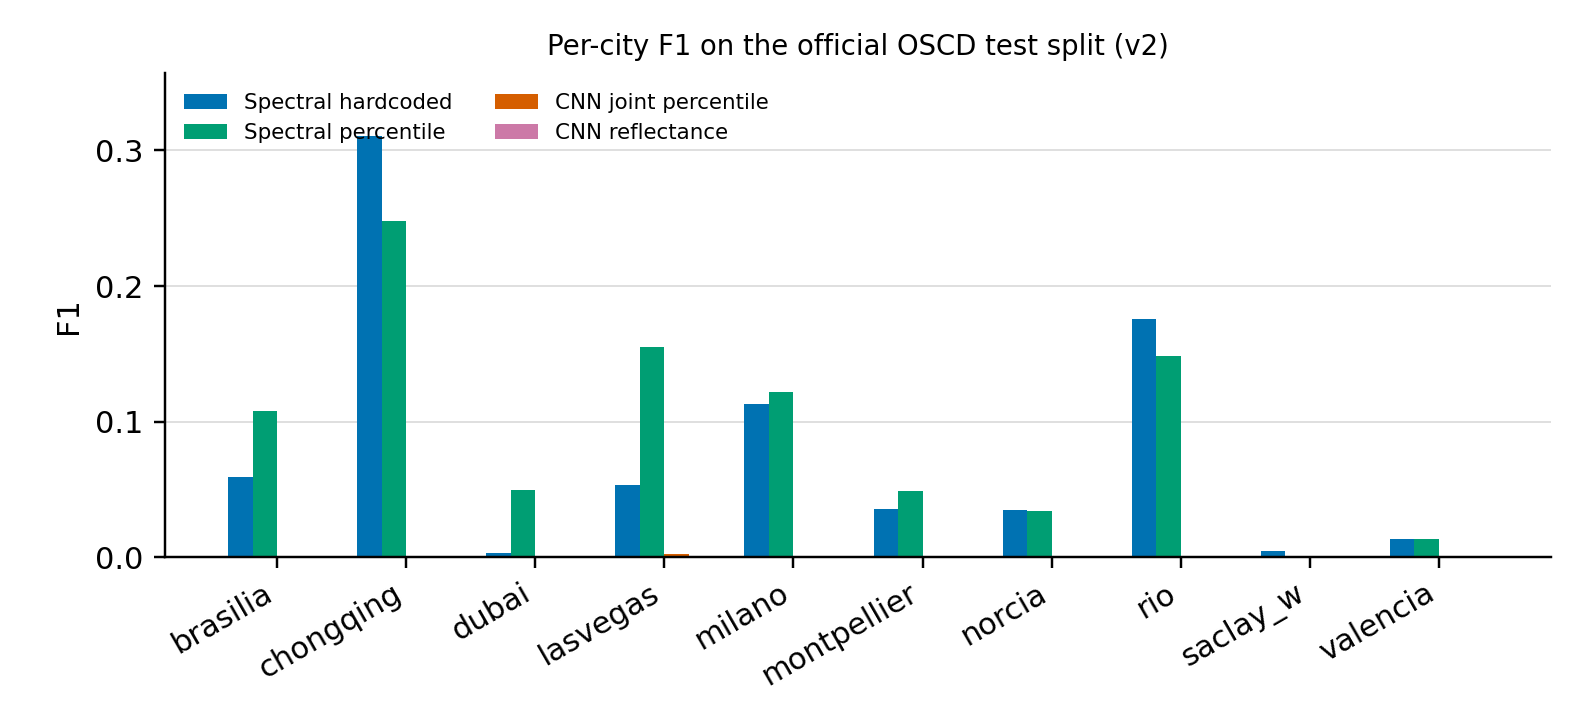
\includegraphics[width=0.92\textwidth]{figures/fig_per_city_f1.png}
\caption{Per-city F1 on the official OSCD test split (v2) for the four
F1-scored methods. Otsu is omitted here because its reported score is overall
accuracy; see Table~\ref{tab:pooled}. City-level variation is large: the
percentile rule ranges from 0.0005 to 0.2481 across the ten cities.}
\label{fig:per-city}
\end{figure*}

\begin{figure}[t]
\centering
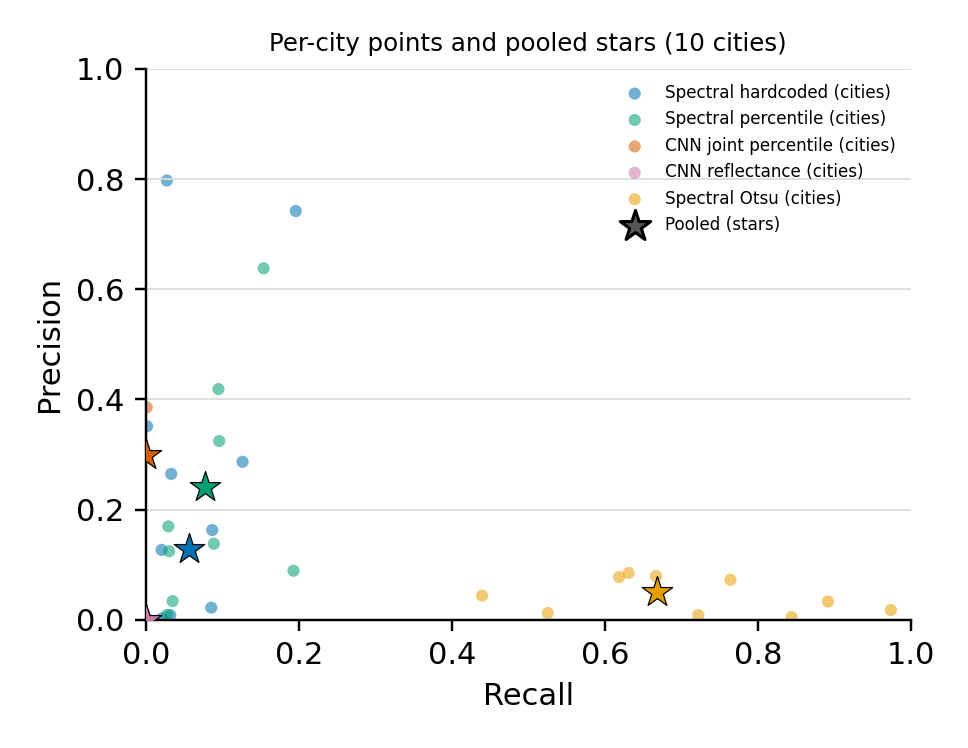
\includegraphics[width=\columnwidth]{figures/fig_precision_recall.png}
\caption{Per-city precision--recall points (small dots) and pooled confusion
counts (stars) for the five configurations. The Otsu star sits at high recall
and low precision; the CNN stars sit at near-zero recall.}
\label{fig:pr}
\end{figure}

\begin{figure*}[t]
\centering
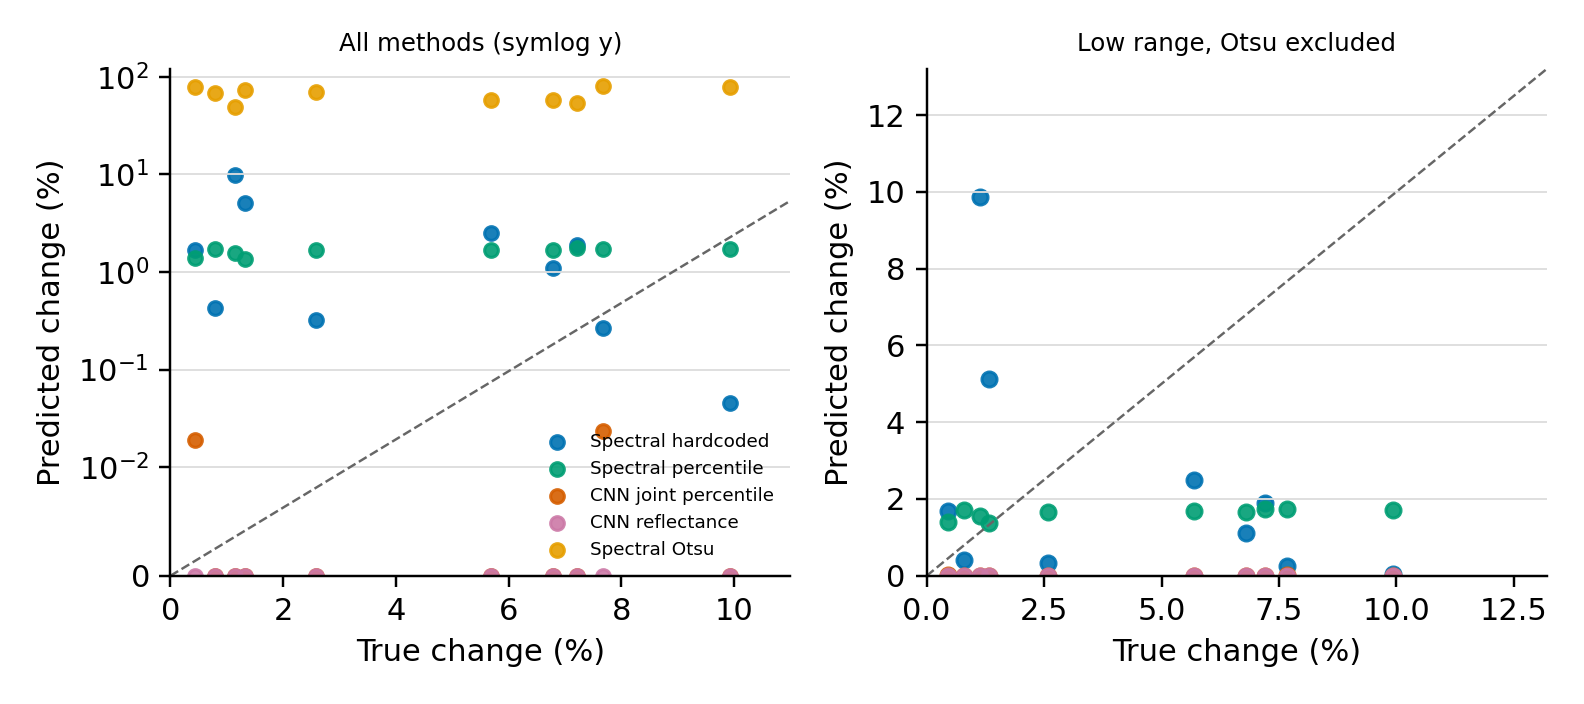
\includegraphics[width=0.95\textwidth]{figures/fig_predicted_vs_true.png}
\caption{Predicted versus true change fractions. Left: all methods with a
symmetric-logarithmic vertical axis; right: the low range with Otsu excluded.
The dashed line is predicted $=$ true. The spectral rules sit below the line,
Otsu sits far above it, and the CNN variants sit on the zero axis.}
\label{fig:fractions}
\end{figure*}

Figure~\ref{fig:per-city} shows that the aggregate F1 masks large city
differences. The percentile rule ranges from 0.0005 (saclay\_w) to 0.2481
(chongqing); the hardcoded rule ranges from 0.0032 (dubai) to 0.3102
(chongqing). Figure~\ref{fig:fractions} makes the calibration-style failure
visible: the rules systematically under-predict change, while Otsu
over-predicts by an order of magnitude. Figure~\ref{fig:pr} shows that no
configuration occupies a high-precision, high-recall region on this test set.

We did not compute confidence intervals or significance tests for these
values. With ten cities and one label source, the numbers should be read as
descriptive benchmark results, not as population estimates.

\section{Ablations and Validation-Only Improvements}
\label{sec:ablations}
The repository includes optional PIF gain/offset matching, temporal median
compositing, morphological cleanup, an MMU and a fixed leave-one-city-out
search. These are covered by synthetic tests and are off by default. The v2
benchmark did not use them, so this paper cannot attribute any test difference
to them.

The 12-system validation search and its component ablations were not run in
this checkout because the OSCD data and learned artifacts are absent. The
generated ablation table therefore contains a single explicit statement that
the ablation was not run, not an estimated value. A planned v3 protocol freezes
four systems and a one-shot test-scoring rule; it remains uncomputed. Until
those runs exist, no validation or test improvement is claimed.

The optional per-pixel histogram-gradient-boosting classifier is likewise
experimental. It is trained only on OSCD training cities, is disabled by
default, and has no test-city score in this checkout. No accuracy figure is
displayed for it in the interface.

\section{Discussion}
\label{sec:discussion}
The main result is a negative one: a CNN trained on 0.5\,m aerial imagery does
not transfer to 10\,m Sentinel-2 urban change in this benchmark. Near-zero
predicted fractions can yield respectable overall accuracy while being useless
for finding change. Reporting F1, predicted fraction and recall together makes
that failure hard to hide. A domain gap between the training imagery and the
target sensor is a plausible explanation, not a causal finding; the experiment
does not isolate resolution, season, label definition or preprocessing.

The spectral rules are transparent but weak. Percentile thresholding improves
pooled F1 over the hardcoded rule, yet both under-predict change and vary
widely by city. The hardcoded thresholds selected at the edge of the search
grid suggest that the grid, not just the data, limits the result. Otsu is not a
drop-in fix: its high recall is bought with very low precision on this class
balance.

For decision support, the practical consequence is that the tool should emit
candidates, masked-area statistics and provenance, not autonomous change
polygons. The interface follows that rule: unvalidated profiles show no
accuracy numbers, the evidence heatmap is labelled as rule magnitude rather
than probability, and every result records scenes, dates, thresholds and
commit.

\subsection{Future Work}
\label{sec:future}
Four evaluations would change the paper from a descriptive benchmark into
useful evidence. A human-in-the-loop study should record whether operators
accept or reject candidate regions, and report precision at a fixed review
budget rather than pixel F1 alone. Agriculture and deforestation profiles need
season-matched labelled polygons; neither profile currently has an accuracy
claim. Road monitoring requires imagery that resolves sub-10\,m features; the
present data cannot support it. Finally, the preregistered v3 protocol should
be run once, with its log and hashes frozen before test access, and reported
whether it improves on the percentile reference or not.

The optional learned classifier, fusion, calibration and auto-improvement
search are implemented but unvalidated. Completing them requires the
training-only log and an independent evaluation; adding them to the default
pipeline before that would create claims the evidence does not support. A
larger, multi-sensor, multi-season evaluation with city-level intervals is the
appropriate next step; another score on the same ten cities is not.
\texttt{docs/paper/FUTURE\_WORK.md} records the concrete tasks and their
dependencies.

\section{Limitations}
\label{sec:limitations}
The evaluation covers ten cities and urban-change labels only. It does not
validate agriculture, deforestation, water or roads. SCL-based cloud/shadow
masking is not evaluated because the benchmark layout lacks SCL. The CNN
comparison uses one trained checkpoint and two preprocessing variants, without
retraining or architecture search. No confidence intervals are reported.
Threshold selection was limited to a small grid, and two test-scoring events
preceded this paper; the earlier preliminary values are disclosed rather than
presented as independent confirmation. The learned classifier, fusion,
compositing and PIF components are implemented but not validated on labels.
Operational, privacy and licensing limits are documented in the repository's
\texttt{docs/LIMITATIONS.md}; notably, the deployed app has no authentication
and stores previews and locations in local history.

\section{Reproducibility and Ethics}
\label{sec:reproducibility}
The source of record is the tracked v2 JSON, whose SHA-256 is recorded in the
figure manifest. The benchmark code, tests, figure generator and manuscript are
in the repository; OSCD imagery, labels and model weights are not
redistributed. The benchmark is deterministic given the saved data and
configuration; threshold selection reads training cities only. The code commit
used for the v2 analysis and this manuscript's numbers is Phase~E commit
\texttt{a6dad9e}; later Phase~F changes are documentation, figures and tests.
The figure generator verifies that all ten
cities contain all five configurations before plotting, so a missing method
fails loudly rather than producing a partial chart.

OSCD labels are used under their dataset terms; a licence review is required
before redistribution or commercial use. OpenStreetMap context is used under
the ODbL. The tool is intended for decision support and civil land-observation
workflows; it is not a targeting or enforcement system, and every exported
region requires human verification.

\section{Conclusion}
We presented an auditable benchmark of a Sentinel-2 change-detection tool on
the official OSCD test split. A training-selected percentile rule achieved
pooled F1 0.1176 and a hardcoded rule 0.0782; Otsu's headline overall accuracy
was 0.3439 at a 67.35\% predicted-change rate; the learned CNN transferred
poorly (F1 0.0007 or lower). The paper reports these outcomes without
post-test tuning, describes a validation-only improvement protocol, and leaves
its one-shot test score uncomputed. The next step is independent labels for
non-urban profiles and a properly powered, multi-sensor evaluation, not another
number on the same ten cities.

\appendix
\section{Per-City Results}
\clearpage
\onecolumn
% Generated by scripts/make_paper_figures.py from the saved v2 JSON. Do not edit by hand.
\begin{longtable}{llrrrrrr}
\caption{Per-city results on the official OSCD test split (v2). Fractions are percentages. Otsu's reported score is OA; its F1 is included for completeness.}\\
\toprule
City & Method & True (\%) & Pred. (\%) & Precision & Recall & F1 & OA \\
\midrule
\endfirsthead
\toprule
City & Method & True (\%) & Pred. (\%) & Precision & Recall & F1 & OA \\
\midrule
\endhead
brasilia & Spectral hardcoded & 2.58 & 0.32 & 0.2648 & 0.0332 & 0.0590 & 0.9727 \\
brasilia & Spectral percentile & 2.58 & 1.66 & 0.1381 & 0.0889 & 0.1082 & 0.9622 \\
brasilia & CNN joint percentile & 2.58 & 0.00 & 0.0000 & 0.0000 & 0.0000 & 0.9742 \\
brasilia & CNN reflectance & 2.58 & 0.00 & 0.0000 & 0.0000 & 0.0000 & 0.9742 \\
brasilia & Spectral Otsu & 2.58 & 69.31 & 0.0332 & 0.8916 & 0.0640 & 0.3272 \\
chongqing & Spectral hardcoded & 7.21 & 1.91 & 0.7420 & 0.1961 & 0.3102 & 0.9371 \\
chongqing & Spectral percentile & 7.21 & 1.74 & 0.6380 & 0.1540 & 0.2481 & 0.9327 \\
chongqing & CNN joint percentile & 7.21 & 0.00 & 0.0000 & 0.0000 & 0.0000 & 0.9279 \\
chongqing & CNN reflectance & 7.21 & 0.00 & 0.0000 & 0.0000 & 0.0000 & 0.9279 \\
chongqing & Spectral Otsu & 7.21 & 53.58 & 0.0849 & 0.6312 & 0.1497 & 0.4831 \\
dubai & Spectral hardcoded & 9.92 & 0.05 & 0.3514 & 0.0016 & 0.0032 & 0.9006 \\
dubai & Spectral percentile & 9.92 & 1.72 & 0.1696 & 0.0293 & 0.0500 & 0.8894 \\
dubai & CNN joint percentile & 9.92 & 0.00 & 0.0000 & 0.0000 & 0.0000 & 0.9008 \\
dubai & CNN reflectance & 9.92 & 0.00 & 0.0000 & 0.0000 & 0.0000 & 0.9008 \\
dubai & Spectral Otsu & 9.92 & 79.13 & 0.0776 & 0.6187 & 0.1379 & 0.2323 \\
lasvegas & Spectral hardcoded & 7.67 & 0.27 & 0.7974 & 0.0276 & 0.0533 & 0.9248 \\
lasvegas & Spectral percentile & 7.67 & 1.74 & 0.4188 & 0.0949 & 0.1548 & 0.9204 \\
lasvegas & CNN joint percentile & 7.67 & 0.02 & 0.3857 & 0.0012 & 0.0024 & 0.9232 \\
lasvegas & CNN reflectance & 7.67 & 0.00 & 0.0000 & 0.0000 & 0.0000 & 0.9233 \\
lasvegas & Spectral Otsu & 7.67 & 80.71 & 0.0726 & 0.7641 & 0.1327 & 0.2334 \\
milano & Spectral hardcoded & 0.80 & 0.42 & 0.1629 & 0.0868 & 0.1133 & 0.9892 \\
milano & Spectral percentile & 0.80 & 1.72 & 0.0891 & 0.1931 & 0.1219 & 0.9779 \\
milano & CNN joint percentile & 0.80 & 0.00 & 0.0000 & 0.0000 & 0.0000 & 0.9920 \\
milano & CNN reflectance & 0.80 & 0.00 & 0.0000 & 0.0000 & 0.0000 & 0.9920 \\
milano & Spectral Otsu & 0.80 & 67.84 & 0.0085 & 0.7222 & 0.0167 & 0.3252 \\
montpellier & Spectral hardcoded & 6.79 & 1.10 & 0.1269 & 0.0206 & 0.0355 & 0.9238 \\
montpellier & Spectral percentile & 6.79 & 1.67 & 0.1244 & 0.0305 & 0.0490 & 0.9195 \\
montpellier & CNN joint percentile & 6.79 & 0.00 & 0.0000 & 0.0000 & 0.0000 & 0.9321 \\
montpellier & CNN reflectance & 6.79 & 0.00 & 0.0000 & 0.0000 & 0.0000 & 0.9321 \\
montpellier & Spectral Otsu & 6.79 & 57.13 & 0.0793 & 0.6670 & 0.1418 & 0.4514 \\
norcia & Spectral hardcoded & 1.32 & 5.14 & 0.0220 & 0.0856 & 0.0350 & 0.9377 \\
norcia & Spectral percentile & 1.32 & 1.37 & 0.0339 & 0.0350 & 0.0345 & 0.9740 \\
norcia & CNN joint percentile & 1.32 & 0.00 & 0.0000 & 0.0000 & 0.0000 & 0.9868 \\
norcia & CNN reflectance & 1.32 & 0.00 & 0.0000 & 0.0000 & 0.0000 & 0.9868 \\
norcia & Spectral Otsu & 1.32 & 72.75 & 0.0177 & 0.9739 & 0.0348 & 0.2850 \\
rio & Spectral hardcoded & 5.69 & 2.51 & 0.2868 & 0.1264 & 0.1755 & 0.9324 \\
rio & Spectral percentile & 5.69 & 1.68 & 0.3245 & 0.0960 & 0.1482 & 0.9372 \\
rio & CNN joint percentile & 5.69 & 0.00 & 0.0000 & 0.0000 & 0.0000 & 0.9431 \\
rio & CNN reflectance & 5.69 & 0.00 & 0.0000 & 0.0000 & 0.0000 & 0.9431 \\
rio & Spectral Otsu & 5.69 & 57.09 & 0.0438 & 0.4395 & 0.0796 & 0.4223 \\
saclay\_w & Spectral hardcoded & 1.14 & 9.88 & 0.0025 & 0.0215 & 0.0045 & 0.8903 \\
saclay\_w & Spectral percentile & 1.14 & 1.56 & 0.0004 & 0.0006 & 0.0005 & 0.9730 \\
saclay\_w & CNN joint percentile & 1.14 & 0.00 & 0.0000 & 0.0000 & 0.0000 & 0.9886 \\
saclay\_w & CNN reflectance & 1.14 & 0.00 & 0.0000 & 0.0000 & 0.0000 & 0.9886 \\
saclay\_w & Spectral Otsu & 1.14 & 48.90 & 0.0123 & 0.5253 & 0.0240 & 0.5116 \\
valencia & Spectral hardcoded & 0.44 & 1.69 & 0.0084 & 0.0320 & 0.0133 & 0.9789 \\
valencia & Spectral percentile & 0.44 & 1.40 & 0.0088 & 0.0279 & 0.0134 & 0.9818 \\
valencia & CNN joint percentile & 0.44 & 0.02 & 0.0000 & 0.0000 & 0.0000 & 0.9954 \\
valencia & CNN reflectance & 0.44 & 0.00 & 0.0000 & 0.0000 & 0.0000 & 0.9956 \\
valencia & Spectral Otsu & 0.44 & 78.25 & 0.0048 & 0.8442 & 0.0095 & 0.2205 \\
\bottomrule
\end{longtable}

\twocolumn

\section{Validation Ablation Table (Not Run)}
% Generated by scripts/make_paper_figures.py from an optional auto-improve log.
\begin{table}[t]
\centering
\caption{Validation-only component ablation on held-out OSCD training cities. Positive $\Delta$F1 means the component helped. This is not a test-set result.}
\label{tab:ablation}
\small
\begin{tabular}{lrrrr}
\toprule
Component & Pairs & Mean $\Delta$F1 & SD & Decision \\
\midrule
\multicolumn{5}{c}{No auto-improve log was present in this checkout; the ablation was not run.} \\
\bottomrule
\end{tabular}
\end{table}


\end{document}
